\chapter{\Lone Adaptive Control Derivation}\label{ch:derivation}

Failures in early adaptive control were largely impart due to a very naive understanding of robustness.  As paralleled in the X-15's robustness issues, Brian Anderson concludes that "it is clear that the identification time scale needs to be faster than the plant variation time scale, else identification cannot keep up" \cite{anderson2005failures}.   

\section{\Lone Adaptive Control}
The \Lone adaptive controller is an evolution of the concepts implemented by \ac{MRAC}.  They are similar approaches designed to model a \ac{LTI} system with unknown constant parameters.  These parameters are adjusted to achieve the desired outcome of the error between the actual plant (system) and the referenced system model (state predictor) to asymptotically approach zero.   Adaptive control attempts to estimate the plant's unknown parameters in situ.  Parameter estimation is done using either direct or indirect architectures.  The indirect architecture attempts to estimate the system's parameters, which could be considered similar to  system identification.  Alternately the easier to implement direct architecture estimates the controller parameters explicitly.  These architectures can be seen below in Figures~\ref{fig:direct_mrac} and \ref{fig:indirect_mrac}.

\begin{figure}[h!]
 \centering
  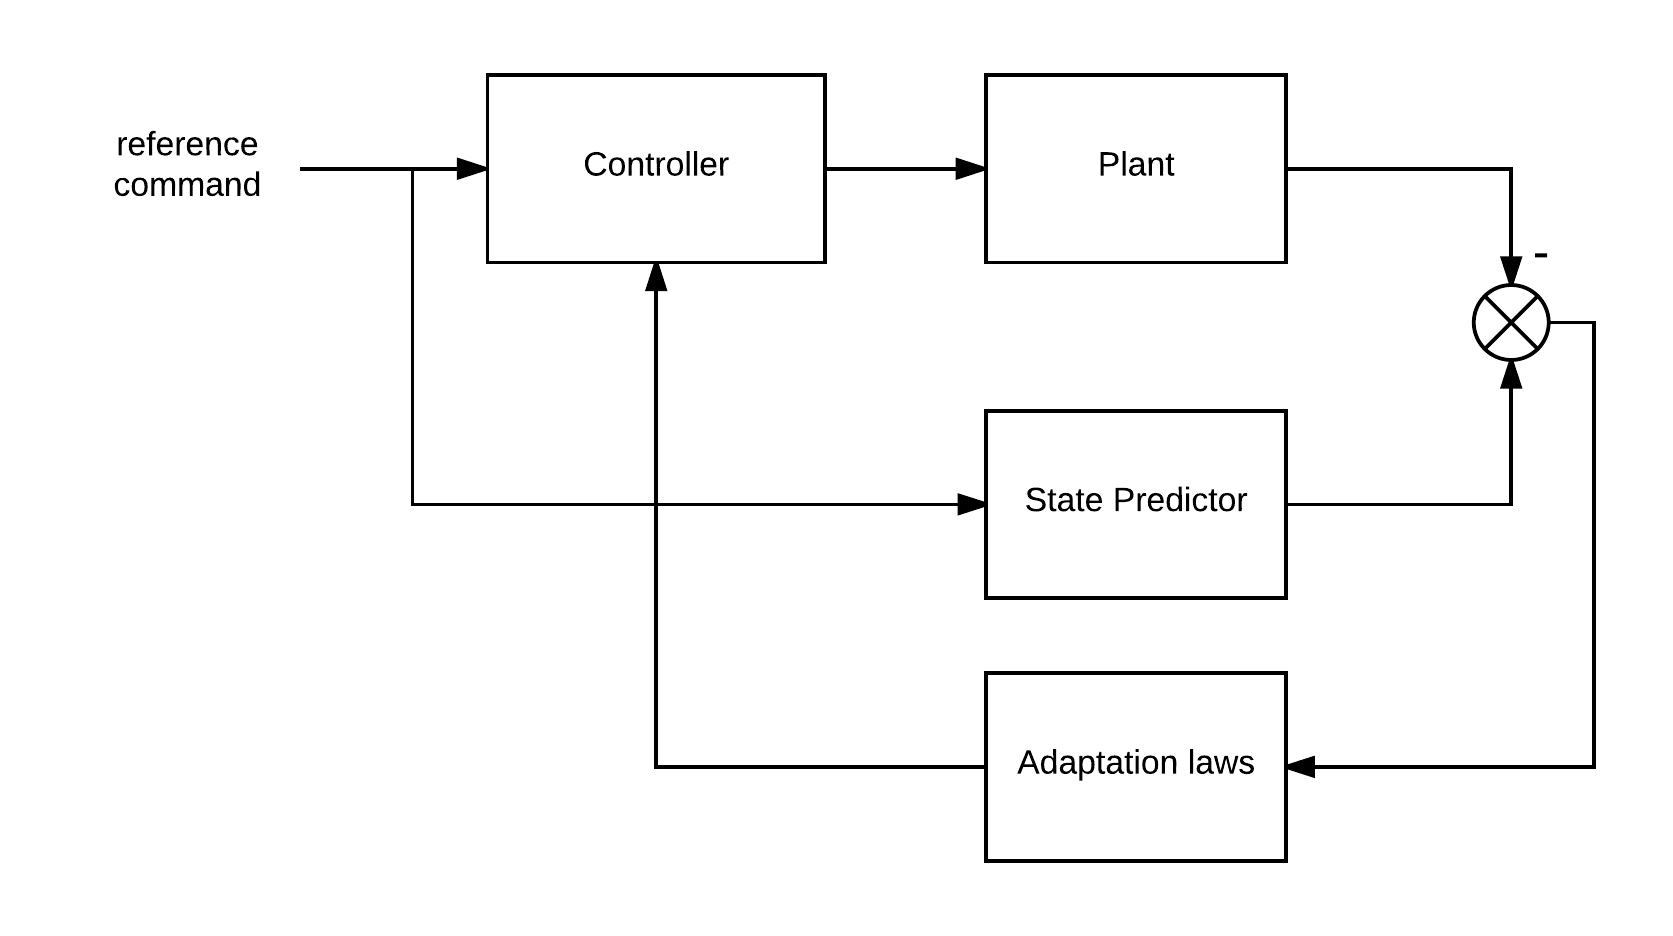
\includegraphics[width=0.65\textwidth]{Direct_MRAC.png}
  \caption{Direct \ac{MRAC} architecture }
  \label{fig:direct_mrac}
\end{figure}

\begin{figure}[h!]
 \centering
  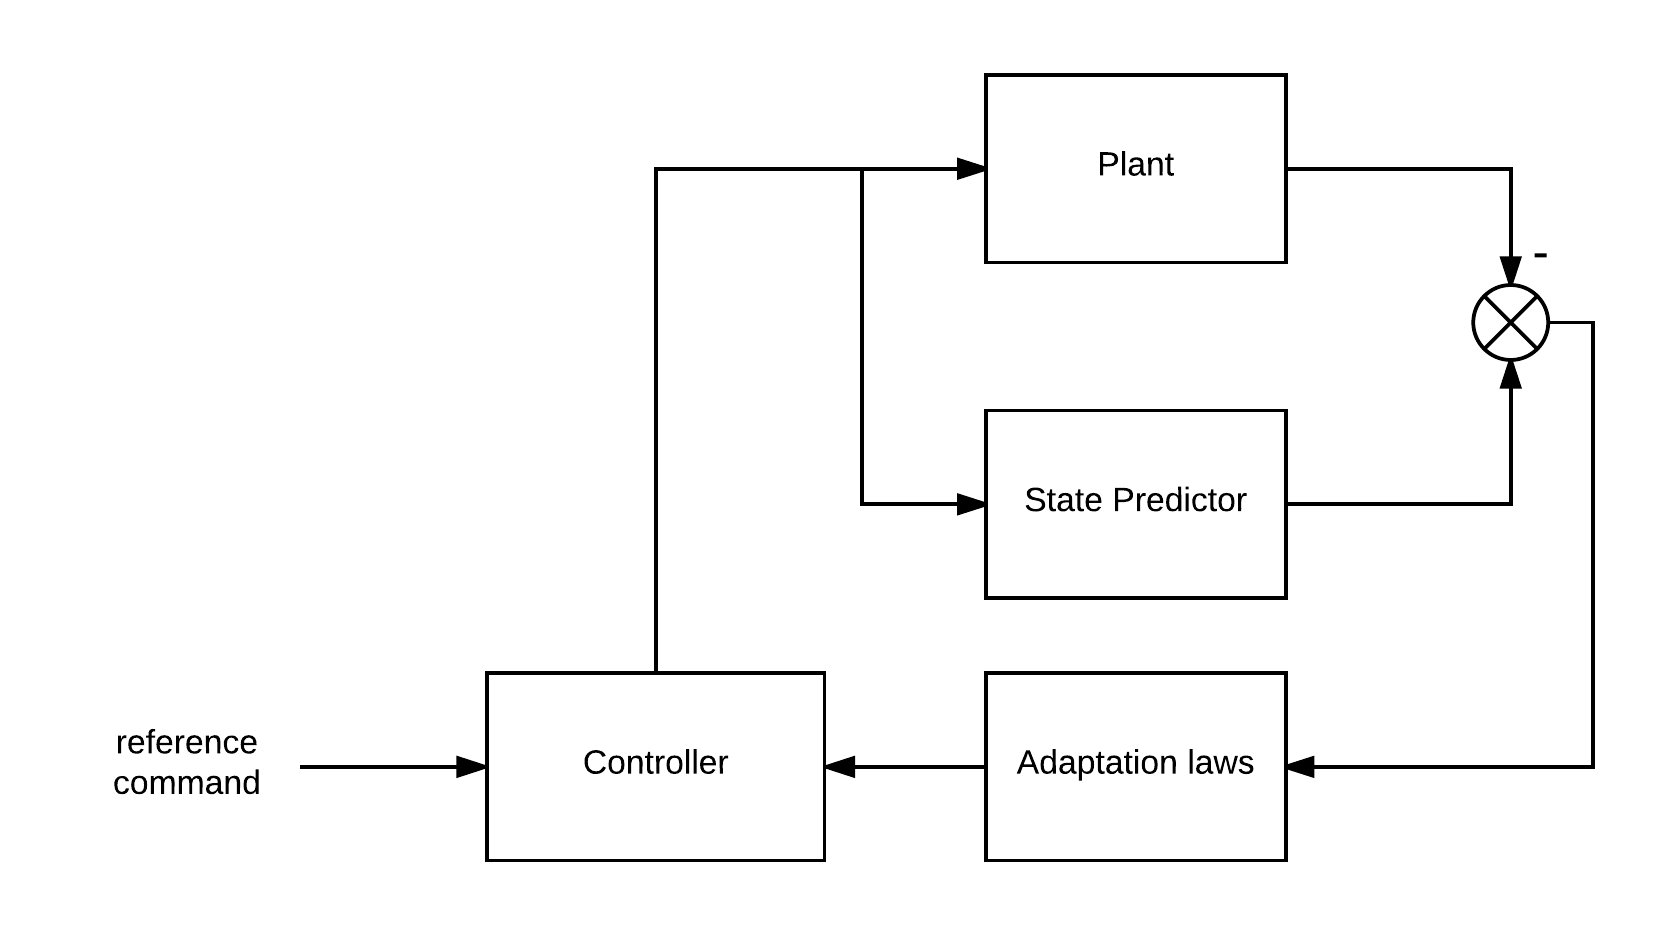
\includegraphics[width=0.65\textwidth]{Indirect_MRAC.png}
  \caption{Indirect \ac{MRAC} architecture }
  \label{fig:indirect_mrac}
\end{figure}

The \Lone adaptive control algorithm asserts that trying to estimate the plant uncertainties outside of the control actuators' bandwidth is overly ambitious.  The system's actuator bandwidth and the slow dynamics of the plant are most commonly the system's limiting factors, and the estimator's robustness/stability could be in question if un-modeled high frequency content exists in the plant.  % See RHORs example here? 
The \Lone adaptive control constrains the objective function by using a low-pass filter (first or second order) to band the frequency response in order to meet robustness specifications.  This low-pass filter should be tuned to a frequency response commensurate with the actuator's frequency response.  When looking at examples of where to place the low-pass filter in the direct and indirect architectures, it becomes clear that the indirect architecture is the only candidate.  Figures~\ref{fig:direct_mrac_lowpass} and \ref{fig:indirect_mrac_lowpass} illustrate the placement of the low-pass filter and its implication on the closed loop model. 

\begin{figure}[h!]
 \centering
  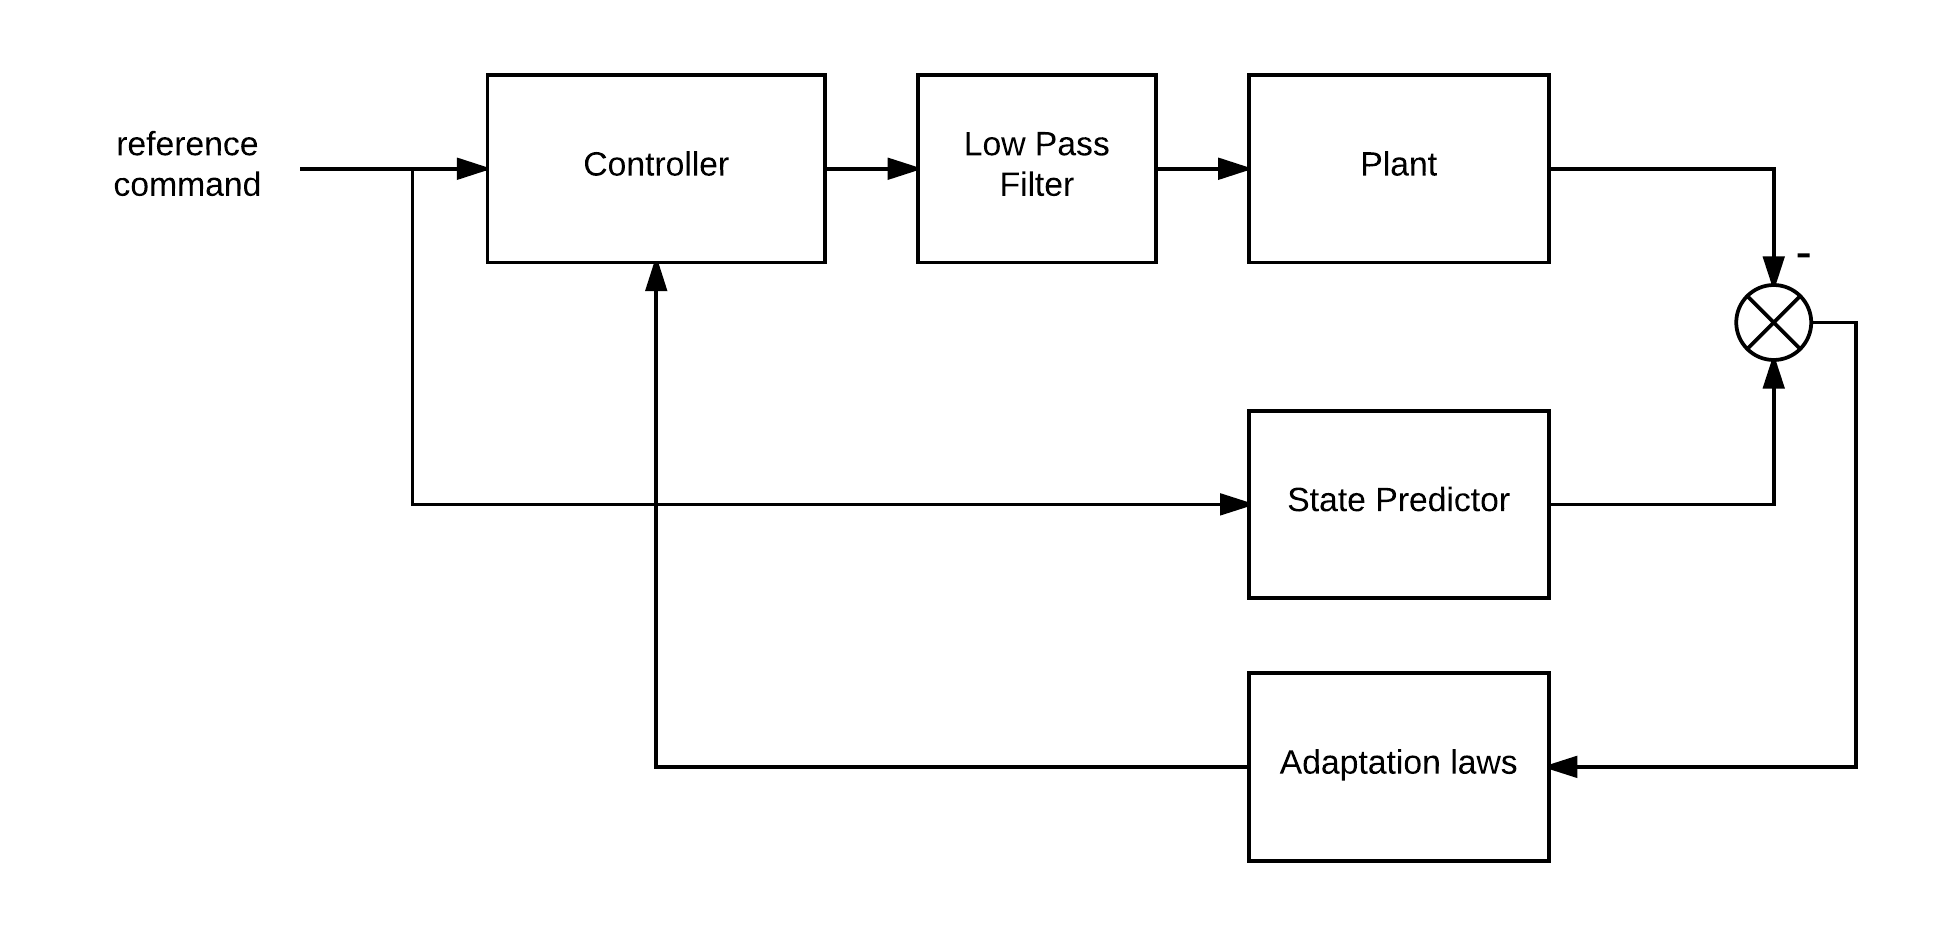
\includegraphics[width=0.65\textwidth]{Direct_MRAC_lowpass.png}
  \caption{Direct \ac{MRAC} architecture with low-pass filter }
  \label{fig:direct_mrac_lowpass}
\end{figure}

\begin{figure}[h!]
 \centering
  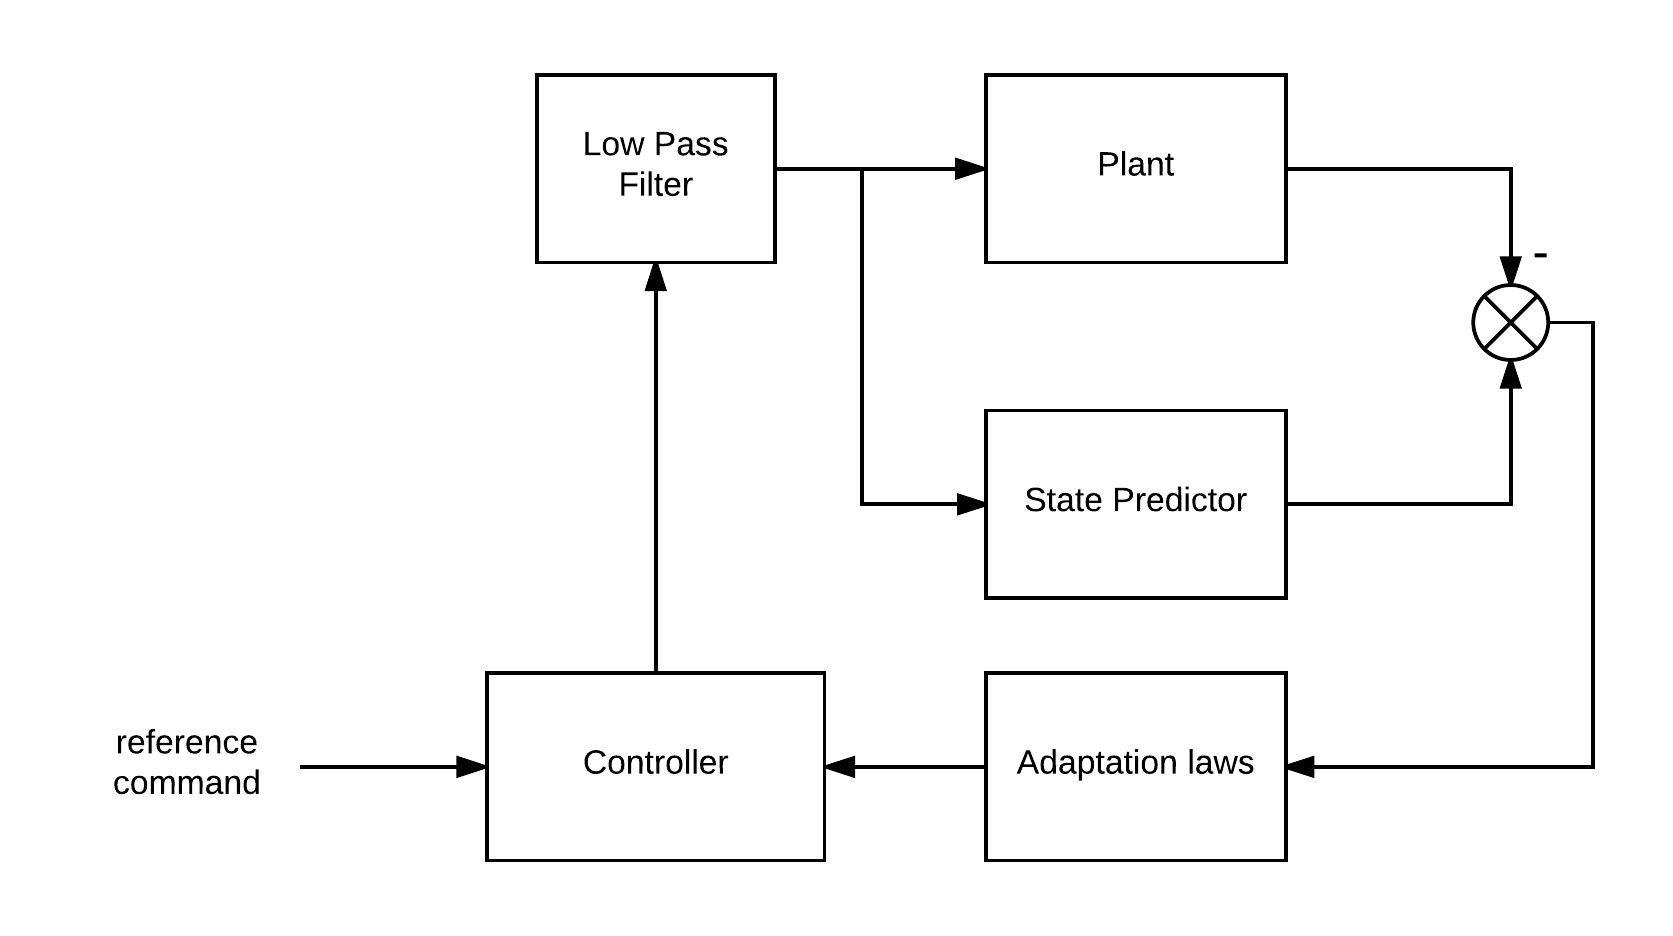
\includegraphics[width=0.65\textwidth]{Indirect_MRAC_lowpass.png}
  \caption{Indirect \ac{MRAC} architecture with low-pass filter }
  \label{fig:indirect_mrac_lowpass}
\end{figure}

 It can be seen that the low-pass filter in the direct architecture inherently changes the structure of the model with the cascading of the low-pass filter and plant block diagrams.  This change mathematically is not mirrored in the state predictor and therefore is not subtractable.  However, in the indirect case, the structure of the model is kept intact and the low-pass filter is applied to both the plant and the state predictor.  This ensures that the low-pass filter is subtractable when calculating the error state and the model's structure is kept intact.

In the primary literature for this research \cite{hovakimyan2010l1}, the author often refers to the state predictor as the reference model or companion model for the direct and indirect architectures respectively.  The reference model (direct architecture) intuitively maps the desired model response to the error feedback.  In the indirect architecture case, the error state is a result of the companion model plus the low-pass filter.  This subtle distinction is necessary because it must be accounted for when tuning the companion model with the included low-pass filter.

Many slight variations of the \Lone adaptive architectures have been derived for various use cases \cite{hovakimyan2010l1}.  Some of the following forms were studied for viability in the fixed wing \ac{UAS} use case:
\begin{itemize}
	\item \ac{SISO} with constant but unknown state parameters
	\item \ac{SISO} with time variant and/or nonlinear unknown state parameters
	\item \ac{MIMO} with constant but unknown state parameters
	\item \ac{MIMO} with time variant and/or nonlinear unknown state parameters
\end{itemize}

\ac{MIMO} control algorithms would potentially afford the controller more ability to cope with system coupling if present.  A fixed wing \ac{UAS} would exhibit coupled behavior due to the coupling present in the aerodynamics but was not chosen due to the added architectural complexity.  Unknown state parameters that are assumed to be constant or time invariant are considered matched uncertainty.  Unknown state parameters that are non-constant (time variant) and/or exhibit non-linear behavior are considered unmatched uncertainty.  The unmatched uncertainty architecture offers a more appealing solution for fixed wing use cases (asymmetric actuator failure, aerodynamic coefficients scaled by dynamic pressure, etc.), but adds a significant amount of complexity to the architecture.  In summary, the \ac{SISO} architecture with matched uncertainty was chosen for this research.  

The \ac{SISO} controller with matched uncertainty was chosen to control pitch rate $(q)$ and roll rate $(p)$ of the aircraft using two separate but parallel controllers.  This meant that the controller could be generalized to a first principles physical point mass model similar to derivations found in rigid body equations of motion.  In this implementation of the \Lone adaptive controller, the desired state $x$ to be controlled was an individual body rate (\eg $q$, $p$). 

\begin{figure}[h!]
 \centering
  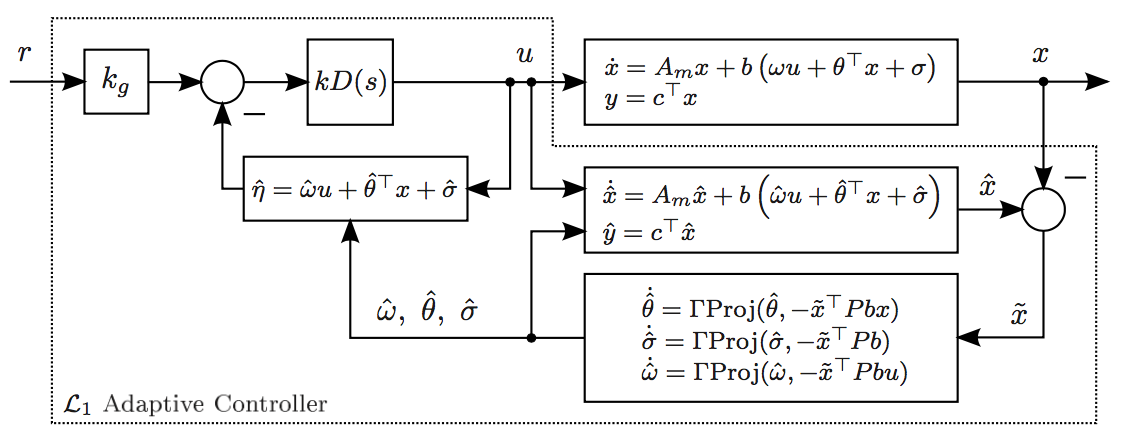
\includegraphics[width=1.0\textwidth]{L1_architecture.png}
  \caption{\Lone Architecture with Matched Uncertainty Block Diagram \cite{hovakimyan2010l1} }
  \label{fig:l1_architecture}
\end{figure}

As seen in Figure~\ref{fig:l1_architecture}, the generalized \Lone architecture in block diagram form and the following elements can be identified:
\begin{itemize}
	\item[] $k_g$ - feed forward input gain
	\item[] $kD(s)$ - user described filter (second order low pass plus integrator)
	\item[] $\hat{\eta}$ - \Lone controller state
	\item[] $\dot{x}$ - first order differential equation of state model
	\item[] $\hat{x}$ - state estimate
	\item[] $\tilde{x}$ - state error
	\item[] $u$ - reference objective
	\item[] $A_m$ - Hurwitz matrix
	\item[] $b$ - input matrix
	\item[] $\hat{\omega}$ - unknown input gain coefficient
	\item[] $\hat{\theta}$ - unknown constant state coefficient
	\item[] $\hat{\sigma}$ - unknown disturbance estimate
	\item[] $\Gamma$ - adaptation gain
	\item[] $Pb$ - solution to the Lyapunov stability criterion	
\end{itemize}

It should also be noted that the architecture presented in Figure~\ref{fig:l1_architecture} includes the use of a projection operator.  The parameters for $\dot{\hat{\omega}}$, $\dot{\hat{\theta}}$, and $\dot{\hat{\sigma}}$ are all projection based adaptation laws.  This simply ensures that the adaptation stays bounded around the feasible region of parameter space.  The Lyapunov stability proofs for this architecture rely on this method to guarantee stability\cite{hovakimyan2010l1} .  More discussion on the specific application of this operator can be found in Appendix [???].

One of the main benefits of using the \ac{SISO} architecture is that the solution to the Lyapunov stability criterion ($Pb$) used in the projection based adaptation laws is greatly simplified.  

In this case, $Pb$ reduces to:
\begin{equation}
Pb = \frac{1}{2\omega_n}
\end{equation}

where $\omega_n$ is the natural frequency in rad/s for the companion model in discrete recursive form assuming DC gain of 1. 


%---------------------------------------------------
\section{\Lone Discrete Time Implementation}







